\documentclass[11pt,twoside]{article}
\usepackage{geometry}
\usepackage{enumerate}
\usepackage{latexsym,booktabs}
\usepackage{amsmath,amssymb}
\usepackage{graphicx}
\usepackage[singlespacing]{setspace}

\usepackage[backend=bibtex]{biblatex}
\addbibresource{literature.bib}

\geometry{a4paper,left=2cm,right=2.0cm, top=2cm, bottom=2.0cm}

\newtheorem{Definition}{Definition}
\newtheorem{Theorem}{Theorem}
\newtheorem{Lemma}{Lemma}
\newtheorem{Corollary}{Corollary}
\newtheorem{Proposition}{Proposition}
\newtheorem{Algorithm}{Algorithm}
\numberwithin{Theorem}{section}
\numberwithin{Definition}{section}
\numberwithin{Lemma}{section}
\numberwithin{Algorithm}{section}
\numberwithin{equation}{section}


\begin{document}

\pagestyle{empty}

% =============================================================================
% Title page
% =============================================================================
\begin{titlepage}
\vspace*{.5em}
\center
\textbf{\large{The School of Mathematics}} \\
\vspace*{1em}
\begin{figure}[!h]
\centering

\includegraphics[width=180pt]{images/CentredLogoCMYK.jpg}
\end{figure}
\vspace{2em}
\textbf{\Huge{Robust Optimisation Monte Carlo for Likelihood-Free Inference}}\\[2em]
\textbf{\LARGE{by}}\\
\vspace{2em}
\textbf{\LARGE{Vasileios Gkolemis}}\\
\vspace{6.5em}
\Large{Dissertation Presented for the Degree of\\
MSc in Operational Research with Data Science}\\
\vspace{6.5em}
\Large{August 2020}\\
\vspace{3em}
\Large{Supervised by\\Senior Lecturer Michael Gutmann}
\vfill
\end{titlepage}

\cleardoublepage

% =============================================================================
% Abstract, acknowledgments, and own work declaration
% =============================================================================
\begin{center}
\Large{Abstract}
\end{center}

Here comes your abstract ...

\clearpage

\begin{center}
\Large{Acknowledgments}
\end{center}

Here come your acknowledgments ...

\clearpage

\begin{center}
\Large{Own Work Declaration}
\end{center}

Here comes your own work declaration

\cleardoublepage



% =============================================================================
% Table of contents, tables, and pictures (if applicable)
% =============================================================================
\pagestyle{plain}
\setcounter{page}{1}
\pagenumbering{Roman}

\tableofcontents
\clearpage
\listoftables
\listoffigures
\cleardoublepage

\pagenumbering{arabic}
\setcounter{page}{1}

\nocite{*}
% \bibliographystyle{abbrv}
\clearpage

\section{Introduction}
\label{sec:introduction}

\subsection{Motivation}

\subsubsection*{\textit{Explanation of Simulation-Based Models}}

A Simulator-Based model is a parameterized stochastic data generating mechanism \cite{Gutmann2016}. The key characteristic is that although we are able to sample (simulate) data points, we cannot evaluate the likelihood of a specific set of observations $y_0$. Formally, a simulator-based model is described as a parameterized family of probability density functions $\{p_{y|\theta}(y)\}_\theta$, whose closed-form is either unknown or intractable to evaluate. Although, evaluating $p_{y|\theta}(y)$ is intractable, sampling is feasible and frequently without huge computational cost. Practically, if we set as $V$ the vector containing the (unobserved) random state of the process, then as a mapping $M(\theta, V) \rightarrow y$

The level of modelling freedom make implicit models particularly captivating; any physical process that can be conceptualized as a computer program of finite (determinstic or stochastic) steps, can be modelled as a Simulator-Based model without any mathematical compromise. This includes any amount of hidden (unobserved) internal variables. On the other hand, this level of freedom comes at a cost; performing inference is particularly demanding from a compuational and mathematical perspective. This constraints the dimensionality of $\theta \in \mathbb{R}^D$ to quite low levels (i.e. $D<20$).

\subsubsection*{\textit{Example}}

For underlying the importance of Simulator-Based models, lets use as example the tuberculosis disease spread model as described in \cite{Tanaka2006}. At each stage we can observe the following events; (a) the transmission of a specific haplotype to a new host (b) the mutation to a different haplotype (c) the exclusion of an infectius host (recovers/dies). The random process, which stops when $m$ infectius hosts are reached, can be parameterized; (a) the transmission rate $\alpha$ (b) the mutation rate $\tau$ and (c) the exclusion rate $\delta$. The outcome of the process is a variable-sized tuple $y_\theta$, containg the size of all different infection groups, as described in figure \ref{fig:tuberculosis_model}. Computing $p(y=y_0|\theta)$ requires tracking all tree-paths that generate the specific tuple along with their probabilities and summing over them. Computing this probability becomes intractable when $m$ grows larger as in real-case scenarios. On the other hand, modeling the data-generation process at a computer program is simple and computationally cheap.

\begin{figure}[!ht]
    \begin{center}
      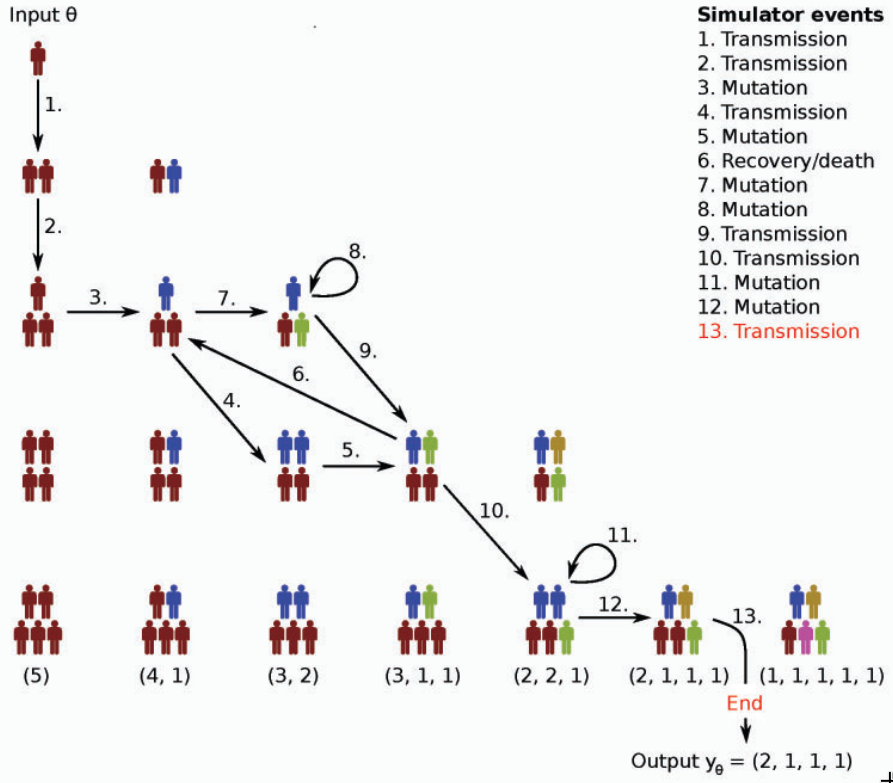
\includegraphics[width=0.49\textwidth]{./images/chapter1/tuber_model_1.png}
      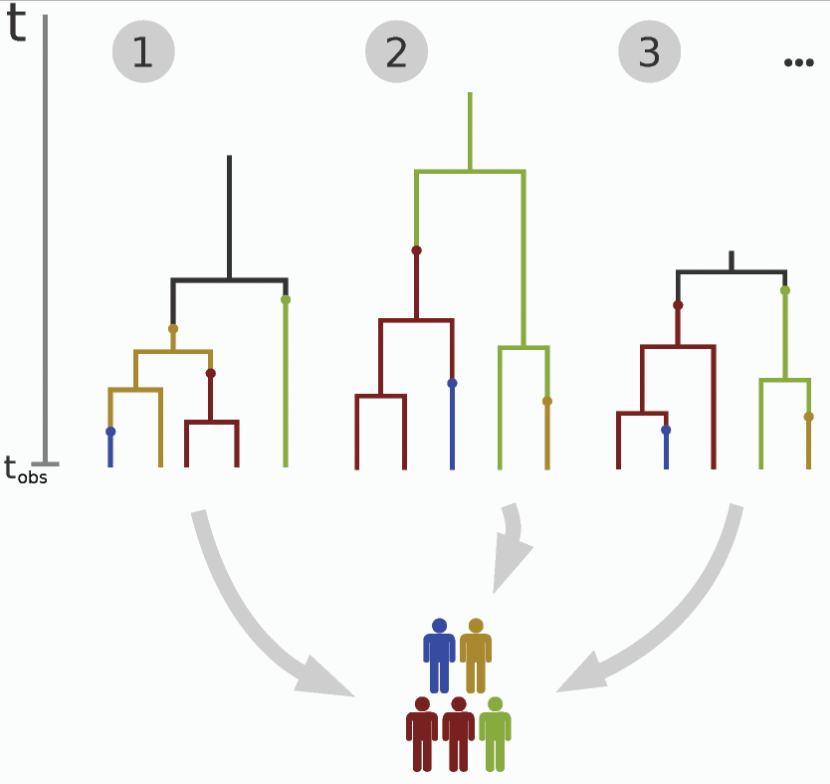
\includegraphics[width=0.42\textwidth]{./images/chapter1/tuber_model_2.png}
    \end{center}
    \caption{Image taken from \cite{Lintusaari2017}}
    \label{fig:tuberculosis_model}
\end{figure}

\subsubsection*{\textit{Goal of Simulation-Based Models}}

As in all Machine Learning (ML) set-ups, the fundamental goal is the derivation of the parameter configuration $\theta^*$ that \textit{describes} well the data (i.e. generates samples $M(\theta^*, V)$ that are as close as possible to the observed data $y_0$). Since Simulation-Based models belong to the broad category of Bayesian Machine Learning, the ultimate goal is to \textit{infer} a posterior distribution $p(\theta|y_0)$ over of all possible configuration set-ups or/and get some samples $\theta \sim p(\theta|y_0)$.

\subsubsection*{\textit{Robust Optimisation Monte Carlo (ROMC) method}}

The ROMC method \cite{Ikonomov2019} is very recent Likelihood-Free approach; its fundamental idea is the transformation of the stochastic data generation process $M(\theta, V)$ to a deterministic function $g(\theta)$, by sampling the variables that the randomness $V_i \sim p(V)$. Hence, we can state that $g(\theta) = M(\theta, V=V_i)$. The ROMC method continues the research line introduced by Meeds et. al \cite{Meeds2015}, by improving some fundamental failure-mode of OMC. ROMC describes a methodology for approximating the posterior through defining and solving deterministic optimisation problems, without enforcing the underlying algorithms for each step; in this sense it can be thought as a meta-algorithm.

\subsubsection*{\textit{Implementation}}

The most important contribution of this work is the implementation of the ROMC method in the Python package Engine for Likelihood-Free Inference (ELFI) \cite{1708.00707}. Since it is very recently published work the ROMC method was not implemented by now in any ML software. This works attempts to provide to the research community a tested and robust implementation for further experimentation.

\subsection{Outline of Thesis}

The remainder of the dissertation is organized as follows. In Chapter 2 we establish the mathematical formulation; more specifically we initially describe the Simulator-Based models and we provide some fundamental algorithms that have been proposed for performing statistical inference. Afterwards, we provide the mathematical description of the ROMC approach \cite{Ikonomov2019}. In Chapter 3, we deal with the implementation part; we initially provide some information regarding the Python package Engine for Likelihood-Free Inference (ELFI) \cite{1708.00707} and subsequently we analyze the implementation details of ROMC in this package. In Chapter 4, we present the functionalities of the ROMC implementation at some real-world examples; this chapter wishes to illustrate the success of the ROMC method and of our implementation at Likelihood-Free tasks. Finally, in chapter 5, we conclude with some thoughts on the work we have done and some future research ideas.

\subsection{Notation}

In this section, we keep an overview of the symbols used throughout the document along with their explanation. We try to keep the notation as consistent as possible, at least to the most central quantities.

\clearpage

\section{Mathematical Modelling}
\label{sec:background}

\clearpage

\subsection{Simulator-Based (Implicit) Models}


\clearpage

\subsection{Robust Optimistation Monte Carlo (ROMC) approach}
\label{sec:Techniques}

Techniques even better because.
\begin{enumerate}
 \item They're magnificent.
 \item If they work.
\end{enumerate}
\clearpage

\subsubsection{Define deterministic optimisation problems}

\subsubsection{Gradient-Based Approach}

\subsubsection{Gaussian Process Approach}

\subsubsection{Weighted Sampling}

\section{Implementation}

Now it's getting very technical \ldots{} I will cite. I will also show my incredible $\alpha$, $\beta$ and $\gamma$ mathematics and do some other fancy stuff.

\subsection{Engine for Likelihood-Free Inference (ELFI) Package}

For example look at this
\begin{equation}\label{eqn:aProblem}
\min{}\sum_{s\in\mathcal{S}}Pr_{s}\left[\sum_{t=1}^{T}\left(
\sum_{g\in\mathcal{G}}\left(\alpha_{gts}C_{g}^{0}+
p_{gts}C_{g}^{1}+\left(p_{gts}\right)^{2}C_{g}^{2}\right)
+\sum_{g\in\mathcal{C}}\gamma_{gts}C_{g}^{s}\right)\right],
\end{equation}
and you will see that it has a little number on the side so that I can refer to it as equation (\ref{eqn:aProblem}). Now if I do this
\begin{eqnarray}
\sum_{i=1}^{n}k_{i}&=&20\label{eqn:one}\\
\sum_{j=20}^{m}\delta_{i}&\geq{}&\eta{}\notag
\end{eqnarray}
I can align two formulae and control which one has a number on the side. It is (\ref{eqn:one}). I can also do something like this
\begin{displaymath}
Y_{l}=\left[\begin{array}{cc}
             \left(y_{s}+i\frac{b_{c}}{2}\right)\frac{1}{\tau{}^{2}} &
             -y_{s}\frac{1}{\tau{}e^{-i\theta^{s}}}\\
             -y_{s}\frac{1}{\tau{}e^{i\theta^{s}}} &
             y_{s}+i\frac{b_{c}}{2}
             \end{array}\right],
\end{displaymath}
and it won't have a number on the side. Now if I have to do some huge mathematics I'd better structure it a little and include linebreaks etc. so that it fits on one page.
\begin{eqnarray}\label{eqn:horrible}
p_{l}^{f}&=&G_{l11}\left(2v_{F(l)}\bar{v}_{F(l)}-\bar{v}_{F(l)}^{2}\right)\\
&+&
\bar{v}_{F(l)}\bar{v}_{T(l)}
\left[
B_{l12}\sin{}(\bar{\delta{}}_{F(l)}-\bar{\delta{}}_{T(l)})
+G_{l12}\cos{}(\bar{\delta{}}_{F(l)}-\bar{\delta{}}_{T(l)})
\right]\notag\\
&+&
\left[\begin{array}{r}
      \bar{v}_{T(l)}
      \left[
      B_{l12}\sin{}(\bar{\delta{}}_{F(l)}-\bar{\delta{}}_{T(l)})
      +G_{l12}\cos{}(\bar{\delta{}}_{F(l)}-\bar{\delta{}}_{T(l)})
      \right]\\
      \bar{v}_{F(l)}
      \left[
      B_{l12}\sin{}(\bar{\delta{}}_{F(l)}-\bar{\delta{}}_{T(l)})
      +G_{l12}\cos{}(\bar{\delta{}}_{F(l)}-\bar{\delta{}}_{T(l)})
      \right]\\
      \bar{v}_{F(l)}\bar{v}_{T(l)}
      \left[
      B_{l12}\cos{}(\bar{\delta{}}_{F(l)}-\bar{\delta{}}_{T(l)})
      -G_{l12}\sin{}(\bar{\delta{}}_{F(l)}-\bar{\delta{}}_{T(l)})
      \right]\\
      \bar{v}_{F(l)}\bar{v}_{T(l)}
      \left[
      -B_{l12}\cos{}(\bar{\delta{}}_{F(l)}-\bar{\delta{}}_{T(l)})
      +G_{l12}\sin{}(\bar{\delta{}}_{F(l)}-\bar{\delta{}}_{T(l)})
      \right]\\
      \end{array}\right]
\cdot{}
\left[\begin{array}{c}
      v_{F(l)}-\bar{v}_{F(l)}\\
      v_{T(l)}-\bar{v}_{T(l)}\\
      \delta_{F(l)}-\bar{\delta{}}_{F(l)}\\
      \delta_{T(l)}-\bar{\delta{}}_{T(l)}
      \end{array}\right],\notag
\end{eqnarray}
This is a lot of fun!
\clearpage

\subsection{Implementation of the ROMC algorithm}
Finally we should have a nice picture like this one. However, I won't forget that figures and table are environments which float around in my document. So LaTeX will place them wherever it thinks they fit well with the surrounding text. I can try to change that with a float specifier, e.g. [!ht].
%This is a comment. The Compiler ignores it. It is here to remind me that, if I use a .jpeg or .png picture file as below I will need to compile the document with the pdflatex compiler.
Now I want to use one of my own environments. I want to define something.
\begin{Definition}
 I define
$$
\Gamma_{\eta}:=\sum_{i=1}^{n}\sum_{j=i}^{n}\xi{}(i,j)
$$
\end{Definition}
I definitely need some good tables, so I do this.
\begin{table}[!ht]
\centering
\begin{tabular}{|ll|rrrr|}
\hline
Case&Generators&Therm. Units&Lines&Peak load: [MW]&[MVar]\\
\hline\hline
6 bus&3 at 3 buses&2&11&210&210\\
9 bus&3 at 3 buses&3&9&315&115\\
24 bus&33 at 11 buses&26&38&2850&580\\
30 bus&6 at 6 buses&5&41&189.2&107.2\\
39 bus&10 at 10 buses&7&46&6254.2&1387.1\\
57 bus&7 at 7 buses&7&80&1250.8&336.4\\
\hline
\end{tabular}
\caption{Something that doesn't make sense.}
\label{tab:things}
\end{table}
I should really refer to Table \ref{tab:things}.

\subsubsection{Training Part}

\subsubsection{Inference Part}

\subsubsection{Inspection Tools}

\subsubsection{Evaluation and Visualisation}

\subsection{Computational Complexity}
% \subsection{And now something else}

% \noindent
% Let:
% \begin{eqnarray*}
% \Omega_0 & = & \{(x,y,z,f): \text{ satisfying } (9)-(19)\}, \\
% \Omega_1 & = & \{(x,y,z,f): \text{ satisfying } (9),(11)-(20)\}, \\
% \overline{\Omega}_0 & = & \{\textbf{0}\leq (x,y,z,f) \leq \textbf{1}: \text{ satisfying } (9)-(18)\}, \\
% \overline{\Omega}_1 & = & \{\textbf{0}\leq (x,y,z,f) \leq \textbf{1}: \text{ satisfying } (9),(11)-(18),(20)\} \,.
% \end{eqnarray*}
% %
% where $\textbf{0}$ and $\textbf{1}$ are vectors of appropriate dimensions with 0's and 1's, respectively.
% Next we see that both $\Omega_0$ and $\Omega_1$ give equivalent formulations for the A-MSSP. In particular, the following statements hold:

% \begin{Proposition}
% $\Omega_0 \subseteq \Omega_1$.
% \end{Proposition}

% \noindent
% \textbf{Proof.}
% Let us suppose there exists $(x,y,z,f) \in \Omega_1$ such that $(x,y,z,f) \notin \Omega_0$.
% Then, there exist indices $i \in I$ and $t \in \{0,\ldots,|T|-s_i\} $ with $x_i^t > \displaystyle 0.5\,\left( \sum_{h=1}^{s_i} x_i^{t+h} +1\right)$.
% By definition, $x_i^t = 1$ and $x_i^{t+h} = 0$ for all $h \in \{1,\dots,s_i\}$. By~(11) and (12), $\displaystyle \sum_{h=1}^{s_i} f_i^{th}=1$, so $f_i^{th'}=1$ for some $h' \in \{1,\dots,s_i\}$.
% But then,
% \[ 0 \:=\: x_i^{t+h'} \:=\: \sum_{h=\max \{1, t+h'-(|T|-s_i)\}}^{\min\{s_i,t+h'\}} f_i^{t+h'-h,h} \:\ge\: f_i^{th'} \:=\: 1 \,,
% \]
% as $h' \in [\max \{1, t+h'-(|T|-s_i)\}, \min\{s_i,t+h'\}]$.
% \hfill $\square$
% \bigskip

% \noindent
% This immediately gives us
% \begin{Corollary}
% AS is a valid formulation for the A-MSSP.
% \end{Corollary}

% \noindent
% Next we compare the Linear Programming (LP) relaxations of the two formulations.

% \begin{Proposition}
% $\overline{\Omega}_1 \subseteq  \overline{\Omega}_0 $.
% \end{Proposition}

% \noindent
% \textbf{Proof.}
% Homework
% \hfill $\square$
% \cleardoublepage


\section{Experiments}
Add experiments ...

\subsection{Higher-Dimension Example}

\subsection{Computational Complexity}
\clearpage

\section{Conclusions}

\subsection{Outcomes}

\subsection{Future Research Directions}
I have no idea how to conclude, so I don't write much. But the stuff that follows is important. lala
\clearpage

\printbibliography
\clearpage

\appendix
\section*{Appendices}
\addcontentsline{toc}{section}{Appendices}

\section{An Appendix}
\label{app:one}

Some stuff.
\clearpage

\section{Another Appendix}
\label{app:two}

Some other stuff.



\end{document}
